%%%%%%%%%%%%%%%%%%%%%%%%%%%%%%%%%%%%%%%%%%%%%%%%%%%%%%%%%%%%%%%%%%%%%%
% LaTeX Template: Designer's CV
%
% Source: http://www.howtotex.com
% 
% Feel free to distribute this example, but please keep the referral
% to HowToTeX.com
% 
% Date: March 2012
%
% Modified by Lim Lian Tze to support multiple pages using fix provided at
% http://www.howtotex.com/templates/creating-a-designers-cv-in-latex/
% Date: November 2014
% Modified for portuguese support by PI. May 2019
%%%%%%%%%%%%%%%%%%%%%%%%%%%%%%%%%%%%%%%%%%%%%%%%%%%%%%%%%%%%%%%%%%%%%%
% How to use writeLaTeX: 
%
% You edit the source code here on the left, and the preview on the
% right shows you the result within a few seconds.
%
% Bookmark this page and share the URL with your co-authors. They can
% edit at the same time!
%
% You can upload figures, bibliographies, custom classes and
% styles using the files menu.
%
% If you're new to LaTeX, the wikibook is a great place to start:
% http://en.wikibooks.org/wiki/LaTeX
%
%%%%%%%%%%%%%%%%%%%%%%%%%%%%%%%%%%%%%%%%%%%%%%%%%%%%%%%%%%%%%%%%%%%%%%

%%%%%%%%%%%%%%%%%%%%%%%%%%%%%%%%%%%%%
% Document properties and packages
%%%%%%%%%%%%%%%%%%%%%%%%%%%%%%%%%%%%%
\documentclass[a4paper,12pt,final]{memoir}

% misc
\renewcommand{\familydefault}{bch}	% font
\pagestyle{empty}					% no pagenumbering
\setlength{\parindent}{0pt}			% no paragraph indentation


% required packages (add your own)
\usepackage{flowfram}										% column layout
\usepackage[top=1cm,left=1cm,right=1cm,bottom=1cm]{geometry}% margins
\usepackage{graphicx}										% figures
%\usepackage{url}											% URLs
\usepackage{hyperref}
\usepackage[usenames,dvipsnames]{xcolor}					% color
\usepackage{multicol}										% columns env.
	\setlength{\multicolsep}{0pt}
\usepackage{paralist}										% compact lists
\usepackage{tikz}
\usepackage[utf8]{inputenc} 
\usepackage{enumitem}     
%%%%%%%%%%%%%%%%%%%%%%%%%%%%%%%%%%%%%
% Create column layout
%%%%%%%%%%%%%%%%%%%%%%%%%%%%%%%%%%%%%
% define length commands
\setlength{\vcolumnsep}{\baselineskip}
\setlength{\columnsep}{\vcolumnsep}

% left frame
\newflowframe{0.3\textwidth}{\textheight}{0pt}{0pt}[left]
	\newlength{\LeftMainSep}
	\setlength{\LeftMainSep}{0.22\textwidth}
	\addtolength{\LeftMainSep}{1\columnsep}
 
% small static frame for the vertical line
\newstaticframe{1.5pt}{\textheight}{\LeftMainSep}{0pt}
 
% content of the static frame
\begin{staticcontents}{1}
\hfill
\tikz{%
	\draw[loosely dotted,color=RoyalBlue,line width=1.5pt,yshift=0]
	(0,0) -- (0,\textheight);}%
\hfill\mbox{}
\end{staticcontents}
 
% right frame
\addtolength{\LeftMainSep}{1.5pt}
\addtolength{\LeftMainSep}{1\columnsep}
\newflowframe{0.7\textwidth}{\textheight}{\LeftMainSep}{0pt}[main01]


%%%%%%%%%%%%%%%%%%%%%%%%%%%%%%%%%%%%%
% define macros (for convenience)
%%%%%%%%%%%%%%%%%%%%%%%%%%%%%%%%%%%%%
\newcommand{\Sep}{\vspace{1.5em}}
\newcommand{\SmallSep}{\vspace{0.5em}}

\newenvironment{AboutMe}
	{\ignorespaces\textbf{\color{RoyalBlue}}}
	{\Sep\ignorespacesafterend}
	
\newcommand{\CVSection}[1]
	{\Large\textbf{#1}\par
	\SmallSep\normalsize\normalfont}

\newcommand{\CVItem}[1]
	{\textbf{\color{RoyalBlue} #1}}


%%%%%%%%%%%%%%%%%%%%%%%%%%%%%%%%%%%%%
% Begin document
%%%%%%%%%%%%%%%%%%%%%%%%%%%%%%%%%%%%%
\begin{document}

% Left frame
%%%%%%%%%%%%%%%%%%%%
%
% Upload your own photo using the files menu
\begin{figure}
	%\hfill
	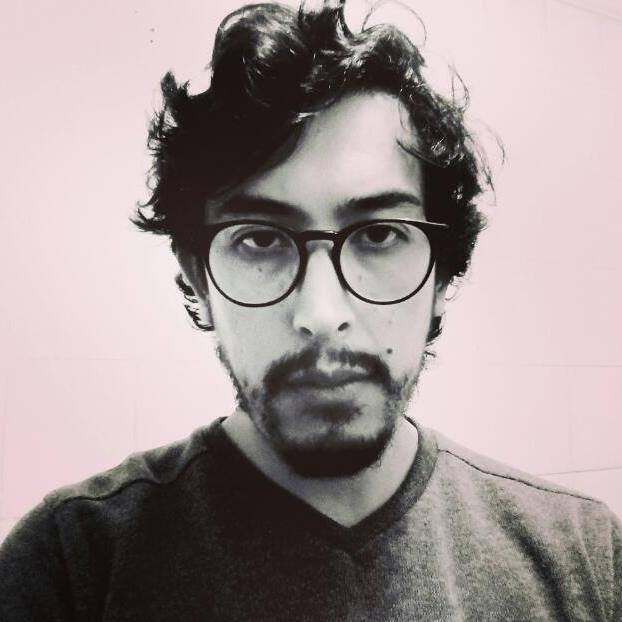
\includegraphics[width=0.75\columnwidth]{my-pic.jpg}
	\vspace{-2cm}
\end{figure}

\begin{flushleft}\small
    \vspace{10mm}
    \textbf{Contato}\\
    \vspace{1mm}
	Pablo Ibieta\\
	\vspace{1mm}
	CPF 235.705.918-40 \\
	\vspace{1mm}
    
\includegraphics[width=0.07\columnwidth]{gmail_icon.png} ibieta.pablo@gmail.com \\
    \vspace{1mm}
    
\includegraphics[width=0.08\columnwidth]{usp_icon.png} pibieta@if.usp.br \\
    
\includegraphics[width=0.07\columnwidth]{cellphone_icon.png} (+55) 11 959 410 565 \\	
	\vspace{4mm}
	\textbf{Endereço Profissional}\\
	\vspace{1mm}
	Rua do Mat\~ao Travessa R\\
	\vspace{1mm}
	Nr. 187, Sala 3096 \\
	\vspace{1mm}
	CEP 05508-090\\
	\vspace{1mm}
	S\~{a}o Paulo, Brasil.\\
	\vspace{4mm}
	\textbf{Endereço Residencial}\\
	\vspace{1mm}
	Rua Frei In\'{a}cio \\
	\vspace{1mm}
	da Concei\c{c}\~{a}o 237, Apto 6 \\
	\vspace{1mm}
	CEP 05362-040 \\
	\vspace{1mm}
	S\~{a}o Paulo, Brasil.\\
	\vspace{4mm}
	\textbf{Detalhes e Publicações}\\
	\vspace{1mm}
	Currículo Lattes: \\
	\vspace{1mm}
	\url{https://bit.ly/2CXGU8i}\\
	\vspace{1mm}
    
\includegraphics[width=0.07\columnwidth]{in_icon.png} /in/pibieta \\
    \vspace{1mm}
    
\includegraphics[width=0.07\columnwidth]{git.jpeg} /pibieta \\
    \vspace{1mm}
    \vspace{4mm}
	\textbf{Idiomas}\\
	\vspace{1mm}
	Espanhol: Nativo\\
	\vspace{1mm}
	Inglês: Fluente\\
	\vspace{1mm}
	Português: Fluente\\
	\vspace{1mm}
\end{flushleft}\normalsize


\framebreak



% Right frame
%%%%%%%%%%%%%%%%%%%%
\Huge\bfseries {\color{RoyalBlue}J. Pablo Ibieta Jimenez} \\
\Large\bfseries Físico \\

\normalsize\normalfont
\vspace{-20pt} 
% About me
\begin{AboutMe}
Doutorando no Instituto de Física da Universidade de São Paulo, desde 2012 atuo como cientista pesquisador na área de Física Quântica. Desenvolvi ferramentas matemáticas e de computação relacionadas com análise de dados, o que envolve manipulação e interpretação dos dados assim como o uso de ferramentas estatísticas para comparar dados com modelos matemáticos. Para complementar esse conjunto de habilidades, atualmente estou focado no estudo e desenvolvimento de ferramentas para Ciência de Dados e Aprendizado de Máquina.   
\end{AboutMe}

\vspace{-20pt} 
% Experience
\CVSection{Experiência}
\CVItem{Set 2012 - presente}\\
\begin{small}
Pesquisador Junior e Monitor,  Instituto de F\'{i}sica, Universidade de S\~{a}o Paulo 
(USP). S\~{a}o Paulo, Brasil. 
Projetos de Pesquisa: 
\end{small}
\begin{footnotesize}
\begin{itemize}[noitemsep,topsep=0pt,parsep=0pt,partopsep=0pt]
\item Fases Topológicas da Matéria, física cuántica e física matemática.
\item Visão Computacional para classificação de imagens Astrofísicas.
\item Processamento de Linguagem Natural e Deep Learning para ChatBots.
\item Análise de Séries Temporais.
\end{itemize}
\end{footnotesize}

\SmallSep

\CVItem{Out 2018 - presente}\\
{\small Kaggle Competitions:}
\begin{footnotesize}
\begin{itemize}[noitemsep,topsep=0pt,parsep=0pt,partopsep=0pt]
\item \emph{New York City Taxi Fare Predictions}.
\item \emph{Predict Future Sales}.
\end{itemize}
\end{footnotesize}
\SmallSep


\CVItem{Jan 2018}\\
{\small Professor Visitante, Universidad Mayor de San Andr\'{e}s, Carrera de Física. La Paz, Bolívia.}
\SmallSep

\CVItem{Set 2005 - Fev 2010}\\
\begin{small}
Pesquisador Junior e Monitor. Instituto de Investigaciones Fisicas,
UMSA, Carrera de Física. La Paz, Bolívia. 
\end{small}
%\SmallSep

\SmallSep

% Education
\CVSection{Educação}
\CVItem{Apr 2015 - May 2019}\\
\begin{small}
 Ph. D. em Física, Universidade de S\~{a}o Paulo (USP).\\ 
S\~{a}o Paulo, Brasil.
 \end{small} 
\SmallSep

\CVItem{2012 - 2015}\\
\begin{small}
M. Sc. em Física, Universidade de S\~{a}o Paulo (USP).\\
S\~{a}o Paulo, Brasil.
\end{small}
\SmallSep

\CVItem{2004 - 2010}\\
\begin{small}
B.Sc. em Física, Universidad Mayor de San Andr\'{e}s (UMSA).\\
La Paz, Bolívia.
\end{small}

\SmallSep

\CVSection{Habilidades}

% Skills

\CVItem{Técnicas}\\
{\small Machine Learning, Neural Networks, Simulations, Feature Engineering, Data Analysis, Visualization, Web.\\}
\vspace{-10pt}
\SmallSep

\CVItem{Desenvolvimento de Software}\\
\begin{small}
Python, R, C, C\texttt{++}, Mathematica, SQL, NoSQL, HTML, CSS.\\
Numpy, Pandas, seaborn, matplotlib, openCV, nltk, spacy, Flask, Django, Tensorflow, Keras, sklearn and XGBoost.\\
\end{small}


% References

%\CVSection{References}

%References upon request.

%%%%%%%%%%%%%%%%%%%%%%%%%%%%%%%%%%%%%
% End document
%%%%%%%%%%%%%%%%%%%%%%%%%%%%%%%%%%%%%
\end{document}